\documentclass[pdflatex,sn-mathphys-num]{sn-jnl}

\usepackage{graphicx}%
\usepackage{multirow}%
\usepackage{amsmath,amssymb,amsfonts}%
\usepackage{amsthm}%
\usepackage{mathrsfs}%
\usepackage[title]{appendix}%
\usepackage{xcolor}%
\usepackage{textcomp}%
\usepackage{manyfoot}%
\usepackage{booktabs}%

\graphicspath{{figures/}}
\raggedbottom

% breakurl works only with pdflatex; other engines set reference URLs with \url
\usepackage{iftex}
\ifPDFTeX\else\AtBeginDocument{\let\burl\url}\fi

\begin{document}

\title[Drift Detection, Diagnosis and Reliability Analysis]{Drift Detection, Diagnosis and Reliability Analysis for Deployed Machine Learning Models}

\author*[1]{\fnm{Rahul} \sur{Guhagarkar}}\email{2023.rahul.guhagarkar@ves.ac.in}
\author[1]{\fnm{Nathan} \sur{Cherian}}
\author[1]{\fnm{Alok} \sur{Pal}}
\author[1]{\fnm{Akul} \sur{Patre}}
\author[1]{\fnm{Sanjay} \sur{Mirchandani}}

\affil*[1]{\orgdiv{Department of Computer Engineering}, \orgname{Vivekanand Education Society's Institute of Technology}, \orgaddress{\street{Hashu Advani Memorial Complex, Collector's Colony, Chembur}, \city{Mumbai}, \postcode{400074}, \country{India}}}

\abstract{Deployed machine learning models lose accuracy when production data drift away from the training data. Monitoring tools raise an alarm when this happens but seldom say what kind of drift occurred, although the right response depends on it: covariate shift calls for reweighting, prior shift for recalibration, concept drift for fresh labels and label noise for a check of the labeling process. This paper presents Data Drift Autopsy, an end-to-end monitoring pipeline that detects drift, estimates the lost accuracy without labels, locates the shifted features, names the drift type, scores the trust due to each prediction and advises whether a cheap retrain will help. At its heart sits a diagnosis made only of hypothesis tests, all held to one family-wise error rate. Its first stage uses no labels and tells covariate shift from prior shift. The second stage is new: given a few hundred late labels, it asks whether the errors have moved in a way the model's own confidence cannot account for, the mark that sets concept drift apart from label noise. With drift injected into two census tasks and two model families, the diagnosis named the type in 85.7 to 94.3\% of windows, ahead of common monitoring rules. A learned meta-classifier did better on drift it had seen, yet fell to 31.1 to 51.2\% on held-out drift mechanisms, where our tests still reached 62.4 to 81.5\%. On four real datasets with documented changes, the pipeline flagged no control window and pointed to the known events.}

\keywords{concept drift, label shift, model monitoring, drift diagnosis, hypothesis testing}

\maketitle


\section{Introduction}\label{sec:intro}

Nobody announces it when a deployed classifier starts to slip. The production data simply wander away from the training data, while the labels that would expose the loss tend to turn up weeks or months later~\cite{rabanser2019failing}. A monitor has to catch the change and make sense of it before those labels exist.

Existing monitors do the first part of that job well. They flag a changed distribution~\cite{rabanser2019failing} and give a fair estimate of how much accuracy has gone~\cite{kivimaki2025performance}. Far fewer say what kind of change took place. That gap matters, since each kind has its own remedy. Moreno-Torres et al.~\cite{moreno2012unifying} distinguish three types of dataset shift. Under covariate shift the inputs drift but the mapping from inputs to labels holds, so reweighting the training data is often enough. Under prior shift it is only the class balance that moves, which recalibration usually fixes. Concept drift alters the mapping itself; nothing short of fresh labels will repair it. To these we add label noise as a fourth type. Here the labels used to grade the model are themselves corrupted, so the fault lies in how labels are collected rather than in the model.

This paper presents Data Drift Autopsy, an end-to-end monitoring pipeline that takes a deployed model, its labeled training data and a stream of unlabeled production data. For every production window it answers the questions a monitoring team asks in turn. Has the data changed? How much accuracy has been lost? Which features moved? What type of drift is it and what probably caused it? The pipeline works for tabular and image models.

The core of the pipeline is the step that names the drift type, which is also the main subject of this paper. Nothing in this step is learned from examples of drift: it is a handful of hypothesis tests that share one significance level and one family-wise error rate. The first stage, which needs no labels, combines existing tools. The second stage is new. It uses a few hundred late labels to ask whether accuracy has dropped and, if so, whether the errors changed in a way that depends on some input feature. Uniform label noise changes the error rate only in line with how confident the model is, while concept drift changes it inside one region of the input space. Because every step is a formal test, the false alarm rate is fixed before the data are seen.

We evaluate the diagnosis on a benchmark of injected drift where the true type is known. We also run the whole pipeline on four real datasets whose changes are documented. The benchmark includes drift mechanisms that the tests were not designed for, so that a method tuned to its own benchmark cannot look good by construction. The contributions are as follows.

\begin{enumerate}
\item An audit test that separates concept drift from label noise using only a few hundred late labels. Existing shift tests, such as DetectShift~\cite{maiapolo2023detectshift}, either need labeled production data or do not consider label noise.
\item A hierarchical procedure that combines this audit with a label-free stage and names four drift types under family-wise error control.
\item A benchmark covering two tabular tasks and two model families, with matched as well as held-out drift mechanisms. It shows that tests built on the definitions of the types carry over to new drift, while a learned rule does not.
\item An end-to-end monitoring pipeline that covers detection, accuracy estimation, localization and diagnosis, evaluated on four real drifts with documented causes.
\end{enumerate}

\section{Related work}\label{sec:sota}

\emph{Drift types.} Moreno-Torres et al.~\cite{moreno2012unifying} define covariate shift, prior shift and concept shift by the part of the joint distribution of inputs and labels that changes. DetectShift tests for a change in this joint distribution and in each of its parts, $P(X)$, $P(Y)$, $P(X\mid Y)$ and $P(Y\mid X)$~\cite{maiapolo2023detectshift}. It needs labels for the new data, however, which its authors acknowledge as a limitation. We keep the same definitions, add label noise as a fourth type and ask for labels only in a small audit.

\emph{Label shift.} Black-box shift estimation (BBSE) recovers the new class prior from the confusion matrix of any classifier~\cite{lipton2018bbse}. It assumes that the inputs inside each class stay as they were, which is exactly the property that separates prior shift from covariate shift. Roschewitz et al.~\cite{roschewitz2025shiftid} test this property on medical images. They resample the reference data to the estimated prevalence and attribute the shift to prevalence if the features then stop differing. Our label-free stage follows the same idea. It differs in two ways: it uses importance weights in place of resampling and it puts every label-free decision into one family with a stated error rate.

In short, each prior method solves part of the problem. To our knowledge, no published method separates concept drift from label noise with a small label audit. Neither has any type diagnosis been tested on drift mechanisms held out from its design.

\section{Method}\label{sec:method}

This section first defines the four drift types precisely and then follows the data through the pipeline introduced in Section~\ref{sec:intro}. Fig.~\ref{fig:architecture} lays out the stages.

\begin{figure}[!htb]
\centering
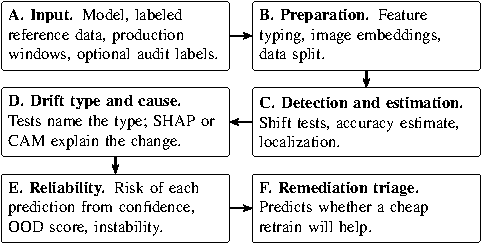
\includegraphics[width=81.6mm,height=0.6\textheight,keepaspectratio]{Fig01.pdf}
\caption{Stages of the monitoring pipeline, from the inputs (A) to the advice on retraining (F). SHAP stands for Shapley additive explanations, CAM for class activation maps and OOD for out-of-distribution}\label{fig:architecture}
\end{figure}

Stages A to C bring the data into a common form, test whether anything has changed and estimate how much accuracy the change may cost. Stage D, the core of the paper, names the type of change and points to its likely cause. Stages E and F act on what was found, first for single predictions and then for the decision to retrain; this paper does not evaluate them. Every decision in the pipeline is a hypothesis test at the significance level $\alpha=0.05$. When many tests are run together, the chance of at least one false alarm is held at $\alpha$ by the Holm procedure~\cite{holm1979}, its weighted form or its Bonferroni bound.

\subsection{Notation and drift types}\label{sec:types}

To test for a drift type we first have to say exactly what that type changes. Write $P(X,Y)$ for the distribution of inputs $X$ and labels $Y$ behind the reference data. A production window (a batch of rows from a later period or from another region) is drawn from $Q(X,Y)$. On every row the model outputs a predicted label $\hat y$ together with a confidence $c$, taken as its largest class probability. The four types differ in what changes between $P$ and $Q$. Covariate shift has $Q(X)\neq P(X)$ while $Q(Y\mid X)=P(Y\mid X)$. Prior shift has $Q(Y)\neq P(Y)$ while $Q(X\mid Y)=P(X\mid Y)$. Concept drift has $Q(Y\mid X)\neq P(Y\mid X)$. Label noise is different again: the true distribution does not move at all, yet each label we observe may have been flipped with some probability. An audit means a random sample of $m$ production rows whose labels come in late. A control window is drawn from the reference distribution itself, so no alarm should fire on it.

\subsection{Reference split, detection and estimation}\label{sec:detection}

Stage C answers three questions: have the data moved, how much accuracy might the change cost and where in the inputs is it located? The labeled reference data are therefore split into three disjoint parts, stratified by class: 60\% for training, 20\% for calibration and 20\% for testing. The model is fitted on the training part alone. The calibration part is the reference window for every detector and fits the accuracy estimator. The test part gives the reference accuracy and doubles as the control window. Images are mapped to the 512-dimensional output of the global average pooling layer of a frozen residual network with 18 layers (ResNet-18) trained on ImageNet~\cite{he2016deep}.

Three detectors decide whether the inputs or the model outputs have moved. The Kolmogorov--Smirnov (KS) test compares each numeric feature, with a Bonferroni correction over features. The maximum mean discrepancy (MMD) test~\cite{gretton2012kernel} compares all standardized inputs jointly through a Gaussian kernel, with a permutation p value. The confidence test compares histograms of $c$ with a $\chi^2$ test of homogeneity.

Labels arrive late, so the accuracy is first estimated from the model's own confidence with confidence-based performance estimation (CBPE)~\cite{kivimaki2025performance}. A map $a(\cdot)$ from confidence to the probability of a correct prediction is fitted by histogram binning on the calibration part. For a window with confidences $c_1$ to $c_n$, the estimate $\hat A$ is given by

\begin{equation}
\hat A = \frac{1}{n}\sum_{i=1}^{n} a(c_i).\label{eq:cbpe}
\end{equation}

\noindent A confidence bin that holds fewer than 5 calibration rows cannot give a reliable accuracy, so predictions in such a bin keep their own confidence in Eq.~(\ref{eq:cbpe}).

An alarm helps more when it also says where the change sits. Localization tests every feature, with KS for numeric features and the $\chi^2$ homogeneity test for nominal ones, under Holm correction. It reports an effect size between 0 and 1 for each feature: the KS statistic or Cramér's $V$. For nominal features it also gives the share of production rows whose category never occurs in the reference.

\subsection{Drift type diagnosis}\label{sec:diagnosis}

Stage D turns an alarm into one of the four types and thereby into a response. It follows the decision path in Fig.~\ref{fig:decision}. The questions in the upper row use no labels and separate covariate shift from prior shift. The lower row separates concept drift from label noise. It runs only when no label-free test rejects and an audit is available.

\begin{figure}[!htb]
\centering
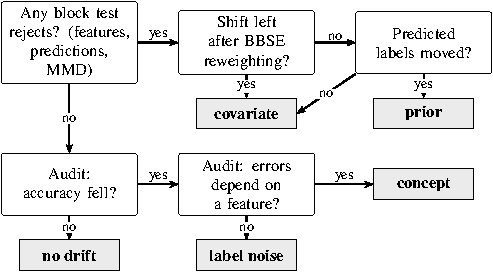
\includegraphics[width=83.5mm,height=0.6\textheight,keepaspectratio]{Fig02.pdf}
\caption{Decision path that names the drift type. Questions are shown in white boxes and verdicts in gray boxes; the upper row needs no labels and the lower row uses the audit}\label{fig:decision}
\end{figure}

\emph{Label-free stage.} The first question is whether anything has moved at all. Three blocks of tests answer it: the feature tests, a $\chi^2$ test on the predicted labels and the MMD test. They form one family tested at level $\alpha$ with a weighted Holm procedure~\cite{holm1979}. A test that rejects hands its weight on to those still waiting, which is how the family-wise error rate survives every label-free decision.

A rejection raises the next question: could a change in the class balance alone produce what we see? To find out, BBSE first estimates the new class prior. Let $C_{jk}=P(\hat y=j,y=k)$ on the calibration part and let $\mu_j$ be the share of production predictions that fall in class $j$. The class weights $w_k=Q(Y=k)/P(Y=k)$ are given by the solution of

\begin{equation}
C\,w = \mu.\label{eq:bbse}
\end{equation}

\noindent If the shift really is a pure prior shift, each class keeps its own input distribution. Reweighting every reference row by the weight $w_{y}$ of its class, as given by Eq.~(\ref{eq:bbse}), ought then to reproduce the production inputs. Checking this is the label shift consistency test, which borrows the prevalence adjustment idea of Roschewitz et al.~\cite{roschewitz2025shiftid}. The feature tests are repeated against the weighted reference. A feature that still differs carries a covariate shift. If no feature differs and the predicted labels have moved, the shift is a prior shift. A prior shift always moves the predicted labels of an informative classifier, so a shift that leaves them in place is called covariate.

\emph{Audit stage.} Concept drift and label noise do not touch the inputs or the model outputs, so only labels can reveal them. The audit draws $m$ late labels and first checks, with a one-sided two-proportion test, whether accuracy has dropped. If it has, the next question is whether the change in errors depends on a feature. To answer it, a logistic model of whether a prediction is correct is fitted on the calibration rows and the audit rows together. Its null form holds 5 confidence bins at reference quantiles, bins of a feature $f$, an audit indicator and the interaction of that indicator with the confidence bins. The alternative adds the interaction of the indicator with the bins of $f$. A likelihood ratio test compares the two for each feature.

The confidence term is what separates the two types. In a binary task, uniform label noise at rate $r$ makes the probability of a correct prediction equal to $r+(1-2r)\,q(x)$, where $q(x)$ is the model's own probability of being right at $x$. The change therefore depends on $x$ only through $q(x)$, which the confidence bins of the null absorb. Concept drift, by contrast, moves the errors inside a region of some feature. A feature that stays significant after Holm correction therefore points to concept drift. If no feature is significant, the verdict is label noise. Each of the two stages is tested at level $\alpha$, so a window without drift receives a drift verdict with probability at most $2\alpha$.

\section{Experimental setup}\label{sec:setup}

The experiments are built around two questions. First, does the procedure name the type correctly when the truth is known, including for drift it was not designed for? Second, does it behave sensibly on real drift, where the type is unknown but the causes are on record?

\emph{Protocol.} Every setting below was fixed before the evaluation that uses it. The diagnosis was frozen before the held-out design B was run for the first time. All randomness is seeded, so every result can be repeated exactly.

\subsection{Models}

A diagnosis that worked for only one kind of model would be of limited use, so the pipeline monitors two untuned model families. The first is logistic regression (LR) with $L_2$ regularization ($C=1$) on standardized numeric and one-hot encoded nominal features. The second is histogram gradient boosting (GB)~\cite{ke2017lightgbm} from scikit-learn~\cite{pedregosa2011scikit} with default settings, no early stopping and native splits on nominal codes. For CLEAR-10 both models work on the frozen embeddings.

\subsection{Datasets}\label{sec:datasets}

The real datasets were chosen because the cause of their drift is documented, which lets us check the verdicts against known events. Two are census tasks from the American Community Survey (ACS) with data from California (CA), Texas (TX), New York (NY), Florida (FL) and Washington (WA). The other two are a gas sensor array and an image stream.

\emph{ACS Income and ACS Employment.} Both tasks come from the ACS of the United States Census Bureau, as packaged by Folktables~\cite{ding2021retiring}. ACS Income predicts from 10 features whether a person earns more than \$50,000. ACS Employment predicts from 16 features whether a person aged 16 to 90 is employed. CA 2014 is the reference. The temporal windows are CA 2015 to 2019 and 2021 to 2023, as no standard 2020 release exists~\cite{census2021experimental}. Five documented changes fall in these years: new occupation codes in 2018~\cite{census2020occupation}, a redesigned relationship question in 2019, a new coding of race answers from 2020~\cite{census2021race}, the pandemic and wage growth against the fixed income threshold.

\emph{Gas sensor array drift.} This dataset from the machine learning repository of the University of California, Irvine (UCI) holds 13,910 measurements of six gases by 16 metal oxide sensors, taken over 36 months in ten batches~\cite{vergara2012gas}. As the sensors age, their response to the same gas drifts while the labels stay exact. This is a documented change in $P(X\mid Y)$. Batches 1 and 2 form the reference and batches 3 to 10 the windows. Some batches are small, so the number of audit labels for a window of $n$ rows is given by $\min(600,\lfloor n/2\rfloor)$.

\emph{CLEAR-10.} This image stream has ten object classes and a background class, spread over ten time-ordered buckets of about 3,300 images each~\cite{lin2021clear}. Bucket 1 is the reference.

\subsection{Injection benchmark}\label{sec:benchmark-setup}

The type of a real drift is never known for certain, so the diagnosis is graded on drift that we inject ourselves. The benchmark uses the 2014 data of 5 states (CA, TX, NY, FL, WA) for both ACS tasks. For each of 10 seeds the split, the window and the injection are drawn again, which gives 50 replicates per configuration. A replicate draws a production window of 4,000 rows and a grading holdout of 2,000 rows from the test part. Each mechanism is injected into both at three intensities. The audit uses 600 labels.

\emph{Design A} injects the four types in ways that partly match how the tests work. Covariate shift rescales two numeric features (ACS Income: AGEP and WKHP) for a random subset of rows. Prior shift drops rows of one class until the positive rate rises by 0.14, 0.23 and 0.32. Concept drift inverts the labels of the 15, 30 and 50\% of rows with the highest value of one feature (ACS Income: SCHL). Label noise flips a random 8, 18 and 32\% of the labels. Each replicate also contains a control window without drift.

\emph{Design B} uses mechanisms that the tests were not built for. Covariate shift becomes selection bias. Each row is kept with a probability given by $\sigma(\beta s(x))$, where $\sigma$ is the logistic function, $s$ is a seeded random score over all inputs and $\beta\in\{0.5, 1, 1.5\}$. The rows stay real and $P(Y\mid X)$ is exactly unchanged. Prior shift lowers the positive rate by 0.08, 0.14 and 0.20. Concept drift inverts the labels in the top 15, 30 and 50\% of a second random score, which marks out an oblique region that no single feature describes. For ACS Income a second concept drift raises the income threshold to \$55,000, \$60,000 and \$70,000. Label noise is class-conditional: positive labels are flipped to negative at rates of 10, 20 and 35\%.

\subsection{Baselines}\label{sec:baselines}

A diagnosis is only worth running if it does better than simpler options. Every method below names one of the five outcomes (no drift or one of the four types) from the same tests and the same audit labels. Three rules stand for current practice. \emph{Input monitoring} reads any input alarm as covariate shift, which is how drift alarms are commonly read. \emph{BBSE first} reads a shift in the predicted labels as prior shift~\cite{lipton2018bbse,rabanser2019failing} and any other alarm as covariate shift. It is our label-free stage without the consistency test. \emph{Error-rate monitoring} also reads a significant drop in audit accuracy as concept drift, as an error-rate detector would~\cite{gama2004ddm}.

The \emph{learned meta-classifier} checks whether a learned rule could replace the tests. It is a GB model trained on nine statistics of each window. In design A it is validated by leaving one state out. In design B it is trained on design A without the state being predicted, so it never sees a held-out mechanism.

Each method is compared with ours through the per-replicate difference in the share of correctly typed windows, tested by sign-flip permutation (10,000 flips) with Holm correction.

\begin{table}[!htb]
\caption{Share of benchmark windows with the correct drift type (\%), for each model family, task and design}\label{tab:methods}%
\begin{tabular}{@{}lrrrr@{}}
\toprule
 & \multicolumn{1}{c}{Inc. A} & \multicolumn{1}{c}{Inc. B} & \multicolumn{1}{c}{Emp. A} & \multicolumn{1}{c}{Emp. B} \\
\midrule
\multicolumn{5}{c}{Logistic regression} \\
\midrule
Ours & 94.3 & 62.4 & 85.7 & 80.5 \\
Input monitoring & 30.3$\downarrow$ & 20.0$\downarrow$ & 30.5$\downarrow$ & 25.0$\downarrow$ \\
BBSE first & 30.5$\downarrow$ & 27.7$\downarrow$ & 30.5$\downarrow$ & 39.2$\downarrow$ \\
Error-rate monitoring & 52.3$\downarrow$ & 48.5$\downarrow$ & 52.2$\downarrow$ & 62.8$\downarrow$ \\
Meta-classifier & 97.5 & 31.1$\downarrow$ & 95.8$\uparrow$ & 48.2$\downarrow$ \\
\midrule
\multicolumn{5}{c}{Gradient boosting} \\
\midrule
Ours & 94.2 & 63.2 & 90.5 & 81.5 \\
Input monitoring & 30.3$\downarrow$ & 20.0$\downarrow$ & 30.5$\downarrow$ & 25.0$\downarrow$ \\
BBSE first & 30.5$\downarrow$ & 28.1$\downarrow$ & 30.6$\downarrow$ & 40.3$\downarrow$ \\
Error-rate monitoring & 52.5$\downarrow$ & 49.6$\downarrow$ & 53.1$\downarrow$ & 64.8$\downarrow$ \\
Meta-classifier & 98.5$\uparrow$ & 39.2$\downarrow$ & 97.4$\uparrow$ & 51.2$\downarrow$ \\
\botrule
\end{tabular}
\end{table}

\section{Results}\label{sec:results}

The benchmark comes first: how often the type is named and whether the procedure carries over to drift it was not designed for. Real drift follows.

\subsection{Drift type against baselines}\label{sec:res-methods}

The most direct test of the diagnosis is how often it names the injected type, compared with the baselines. Table~\ref{tab:methods} gives this share for every configuration, each with 50 replicates.

Inc. and Emp. stand for ACS Income and ACS Employment. A and B are the two designs. An arrow marks a method that differs significantly from ours after Holm correction: a down arrow means that ours is better and an up arrow that ours is worse.

With LR on ACS Income, our procedure names the type in 94.3\% of design A windows (95\% interval [92.3, 95.8]). The best rule baseline reaches 52.3\%. The rules are held back by design, since each can name only some of the five outcomes. Over all eight configurations our procedure is significantly better in 28 of the 32 comparisons with a baseline or the learned rule. It is significantly worse in 3, all against the learned meta-classifier on design A (ACS Employment LR, ACS Income GB and ACS Employment GB).

On design A the learned meta-classifier is the strongest competitor. Validated on states it has not seen, it reaches 97.5\% on ACS Income, above our 94.3\%. The held-out mechanisms of design B turn this around. Trained on design A, the meta-classifier drops to 31.1\% on ACS Income and 48.2\% on ACS Employment, while our procedure keeps 62.4\% and 80.5\%. The learned rule had tied each type to the size and shape of the injected shift. It had learned, for example, that covariate shift means a large shift in two features. It therefore misses selection bias, which moves many features a little. This is the main argument for tests over a learned rule. The tests encode what the drift types are, not what the training examples happened to look like.

Design B has no control windows, so false alarms are measured on design A. Our procedure raised one on 13 of 200 control windows (6.5\%), 7 in the label-free stage and 6 in the audit. That is below the bound of 10\% derived in Section~\ref{sec:diagnosis}.

\subsection{Held-out mechanisms}\label{sec:res-mechanisms}

Design B asks whether the procedure carries over to drift it was not built for. It is the harder of the two tests, since none of its mechanisms shaped any part of the procedure.

Three of the five mechanisms carry over well. Selection bias is named covariate shift in 99\% of ACS Income windows with LR, even though no value is distorted and the shift is spread across all features. A lower positive rate is named prior shift in 92\%. Concept drift in an oblique region, which no single feature bounds, is still recognized in 95\%.

The other two mechanisms are harder. A higher threshold relabels some rows in each window, yet model accuracy hardly moves (mean drop \textminus{}0.3 points). With almost nothing lost, the audit stops at its first question and reports no drift in 132 of the 150 windows. This is intended, as the procedure looks for drift that costs accuracy and this drift costs almost none. Class-conditional label noise is recognized in only 21\% of ACS Income windows, for two reasons. At low flip rates the loss of accuracy is too small to show up in 600 labels. At high rates the errors follow the true class, which is itself correlated with the features, so the error structure test reads the pattern as concept drift. A null model built on confidence alone cannot separate the two, a true limitation. Neither failure involves the label-free stage.

\subsection{Real drift}\label{sec:res-real}

On real data the type of drift is not known, but its causes are on record. Here we ask whether the verdicts agree with those causes and whether the control windows stay quiet.

ACS Income shows the clearest trend, so we start there. Its accuracy falls over time for both models, with LR going from 0.824 in 2015 to 0.749 in 2023, while the CBPE estimate falls far less.

Neither model raises an alarm on the control window. Both call CA 2015, whose accuracy did not change significantly, no drift and every other window covariate shift. The documented events can be read off the localization. The 2018 revision of the occupation codes left 26.6\% of rows with a code that never occurred in 2014. Relationship moves in 2019 (effect size 0.091), when its survey question was redesigned. Race moves from 2021 (effect size 0.186), once the Census Bureau had changed its coding of written race answers~\cite{census2021race}. Wage growth, measured against a fixed income threshold, shows up in the labels instead: their positive share rises from 0.355 in the control window to 0.498 in 2023 while the model predicts only 0.338. Part of the 2023 loss comes from a change in what the labels mean, something no label-free test can detect.

The cost of a drift differs widely between datasets. On ACS Employment every window is diagnosed as covariate shift, yet LR accuracy never changes by more than 2.2 points; relationship (2019) and race (from 2021) shift there as well while the model barely responds. The gas sensor batches all come out as covariate shift too, as they should for aging sensors that alter $P(X\mid Y)$. BBSE at first takes each gas batch for a prior shift, since the predicted labels move too. The consistency test corrects this: the sensors respond differently to a gas mix that has not changed.

CLEAR-10 drifts more gently: buckets 2 and 3 show no drift for either model, while buckets 4, 5, 6, 7, 8, 9 and 10 show covariate shift. In buckets 4, 5, 6 and 9 no single embedding dimension shifts significantly with LR. Only the MMD test sees the change while the predicted labels stay put, which is why the multivariate block is needed.

\section{Discussion and conclusions}\label{sec:discussion}

This paper showed that hypothesis tests with a stated error rate can name the drift type, which decides the right response, from label-free tests and a few hundred late labels. On injected drift the procedure beats rules from monitoring practice and the label shift literature and works for both model families. Unlike a learned meta-classifier, it also carries over to held-out drift, because the tests encode the definitions of the types. On real drift it reported no drift on any control window and traced documented events, from new occupation codes to aging sensors.

Several limits apply. Each benchmark window holds a single type, while real windows such as ACS Income 2023 mix several. The four types are also an idealization: sensor aging changes $P(X\mid Y)$ and, through it, $P(Y\mid X)$, yet our procedure reports it as covariate shift. Design B reduces, but cannot remove, the risk that the benchmark favors the tests. The weighted residual tests do not account for the sampling error of the BBSE weights. At several hundred thousand rows almost any shift is significant, so each decision carries an effect size. The audit lets through drift that does not hurt accuracy and often mistakes class-conditional label noise for concept drift. Deep models trained end to end, text and streaming data remain untested. The next steps are an audit conditioned on the full model output, a model of the sampling error of the BBSE weights and benchmark windows that mix several types.

\bibliography{references}

\end{document}
